\begin{figure*}[th]
  \centering
  \begin{subfigure}[b]{0.49\textwidth}
    \centering
    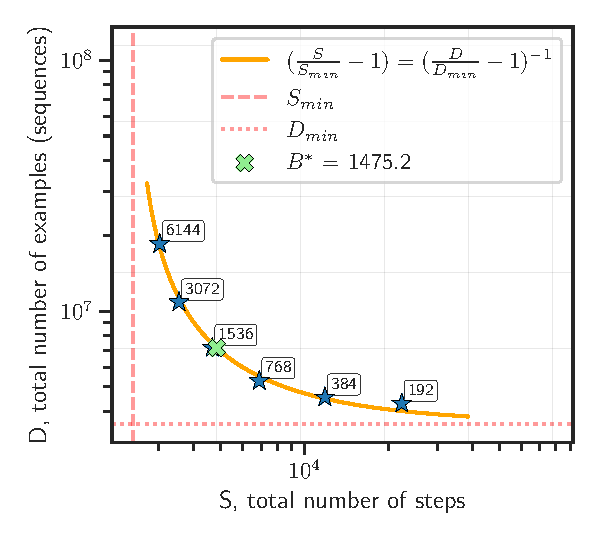
\includegraphics[trim={0.3cm 0.4cm 0.3cm 0.3cm}, clip, width=\linewidth]{pdffigs/loss_data.241005_batchsizes.111M.l=2.872.cbs.pdf}
    \caption{111M, loss=2.872}
    \label{fig:quad_cbs_fits_111M}
  \end{subfigure}
  \hfill
  \begin{subfigure}[b]{0.49\textwidth}
    \centering
    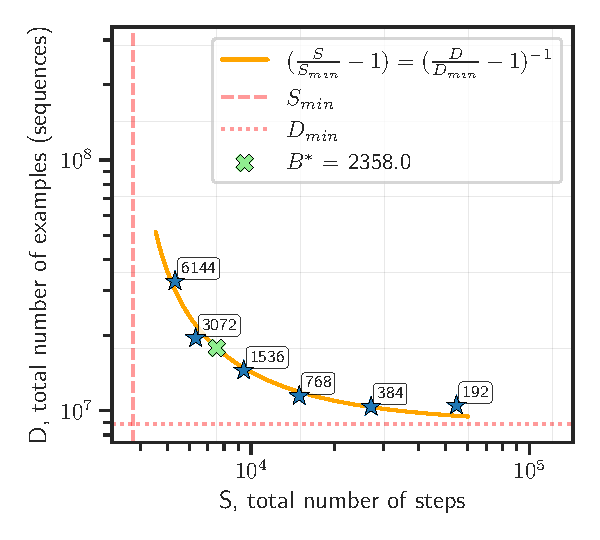
\includegraphics[trim={0.3cm 0.4cm 0.3cm 0.3cm}, clip, width=\linewidth]{pdffigs/loss_data.241005_batchsizes.266M.l=2.600.cbs.pdf}
    \caption{266M, loss=2.600}
    \label{fig:quad_cbs_fits_266M}
  \end{subfigure}
  % Next row
  \begin{subfigure}[b]{0.49\textwidth}
    \centering
    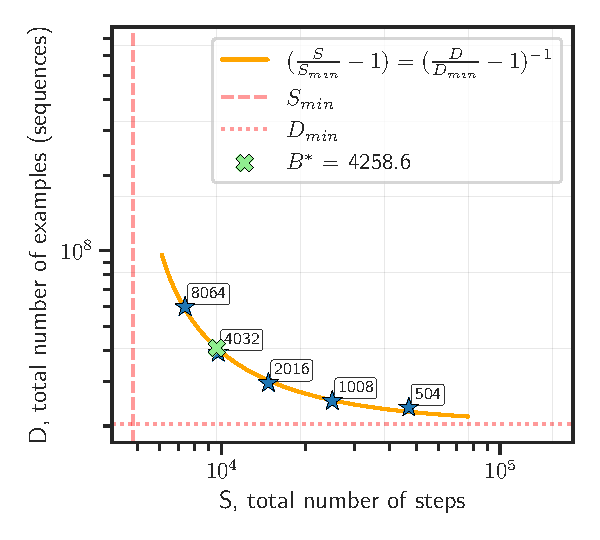
\includegraphics[trim={0.3cm 0.4cm 0.3cm 0.3cm}, clip, width=\linewidth]{pdffigs/loss_data.241005_batchsizes.610M.l=2.437.cbs.pdf}
    \caption{610M scale, loss=2.437}
    \label{fig:quad_cbs_fits_617M}
  \end{subfigure}
  \hfill
  \begin{subfigure}[b]{0.49\textwidth}
    \centering
    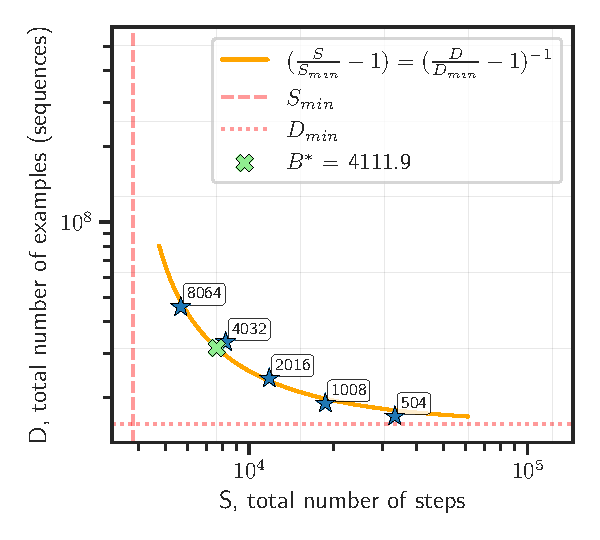
\includegraphics[trim={0.3cm 0.4cm 0.3cm 0.3cm}, clip, width=\linewidth]{pdffigs/loss_data.241005_batchsizes.1.7B.l=2.295.cbs.pdf}
    \caption{1.7B scale, loss=2.295}
    \label{fig:quad_cbs_fits_1_7B}
  \end{subfigure}
  \caption{\textbf{Example fits of trade-off \cref{eq:tradeoff}
      plotting $\smin$ and $\dmin$}: The empirical data has a good fit
    with \cref{eq:tradeoff} across model scales and loss targets.
    These estimates of $\cbs$ are used in fitting the $\cbs$-scaling
    power law
    (\cref{fig:hook} $\rightfig$).\label{fig:quad_cbs_fits}}
\end{figure*}
